\documentclass[border=10pt]{standalone}
\usepackage{pgfplots}
\pgfplotsset{compat=1.18}
\usetikzlibrary{arrows.meta,shapes,calc}

\begin{document}
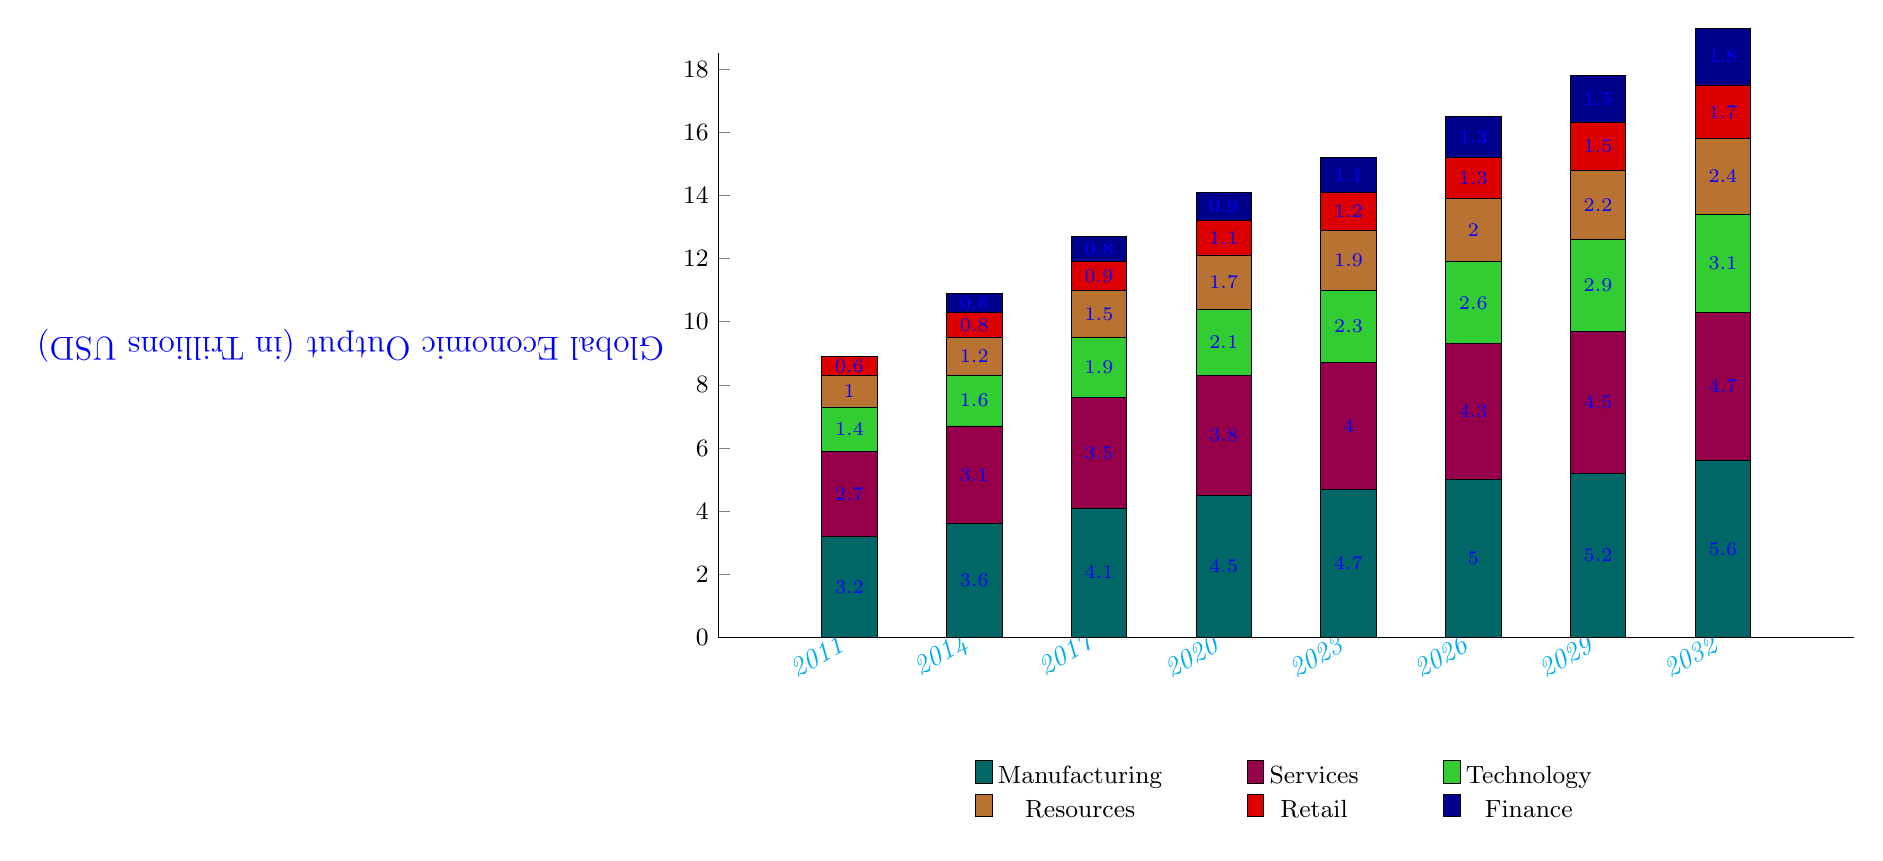
\begin{tikzpicture}
\definecolor{manucolor}{RGB}{0,102,102}     % dark teal
\definecolor{servcolor}{RGB}{150,0,75}      % dark magenta
\definecolor{techcolor}{RGB}{50,205,50}     % bright green
\definecolor{rescolor}{RGB}{184,115,51}     % brown/orange
\definecolor{retcolor}{RGB}{220,0,0}        % red
\definecolor{fincolor}{RGB}{0,0,139}        % dark blue

\begin{axis}[
    width=16cm,
    height=9cm,
    ybar stacked,
    bar width=20pt,
    ymin=0,
    ymax=18.5,
    enlarge x limits=0.15,
    axis x line*=bottom,
    axis y line*=left,
    ymajorgrids=false,
    xtick=data,
    symbolic x coords={2011,2014,2017,2020,2023,2026,2029,2032},
    xticklabel style={
        rotate=30,
        anchor=east,
        text=cyan,
        font=\itshape
    },
    ylabel={\textcolor{blue}{Global Economic Output (in Trillions USD)}},
    ylabel style={rotate=90,align=center,font=\large},
    ytick={0,2,4,6,8,10,12,14,16,18},
    yticklabel style={font=\small},
    legend style={
        at={(0.5,-0.2)},
        anchor=north,
        legend columns=3,
        /tikz/every even column/.append style={column sep=1cm},
        draw=none,
        font=\small
    },
    every axis plot post/.style={
        draw=black,
        line width=0.3pt
    },
    nodes near coords,
    nodes near coords style={
        anchor=center,
        font=\scriptsize,
        text=blue
    },
    clip=false
]

% Data taken from visible labels in the image
% Manufacturing
\addplot+[fill=manucolor] coordinates {
    (2011,3.2) (2014,3.6) (2017,4.1) (2020,4.5)
    (2023,4.7) (2026,5.0) (2029,5.2) (2032,5.6)
};
\addlegendentry{Manufacturing}

% Services
\addplot+[fill=servcolor] coordinates {
    (2011,2.7) (2014,3.1) (2017,3.5) (2020,3.8)
    (2023,4.0) (2026,4.3) (2029,4.5) (2032,4.7)
};
\addlegendentry{Services}

% Technology
\addplot+[fill=techcolor] coordinates {
    (2011,1.4) (2014,1.6) (2017,1.9) (2020,2.1)
    (2023,2.3) (2026,2.6) (2029,2.9) (2032,3.1)
};
\addlegendentry{Technology}

% Resources
\addplot+[fill=rescolor] coordinates {
    (2011,1.0) (2014,1.2) (2017,1.5) (2020,1.7)
    (2023,1.9) (2026,2.0) (2029,2.2) (2032,2.4)
};
\addlegendentry{Resources}

% Retail
\addplot+[fill=retcolor] coordinates {
    (2011,0.6) (2014,0.8) (2017,0.9) (2020,1.1)
    (2023,1.2) (2026,1.3) (2029,1.5) (2032,1.7)
};
\addlegendentry{Retail}

% Finance
\addplot+[fill=fincolor] coordinates {
    (2011,0.0) (2014,0.6) (2017,0.8) (2020,0.9)
    (2023,1.1) (2026,1.3) (2029,1.5) (2032,1.8)
};
\addlegendentry{Finance}

\end{axis}
\end{tikzpicture}
\end{document}